\documentclass[10pt]{article}

\usepackage[applemac]{inputenc}
\usepackage[english]{babel}
\usepackage[T1]{fontenc}
\usepackage{cite, url,color} % Citation numbers being automatically sorted and properly "compressed/ranged".
%\usepackage{pgfplots}
\usepackage{graphics,amsfonts}
\usepackage[pdftex]{graphicx}
\usepackage[cmex10]{amsmath}
% Also, note that the amsmath package sets \interdisplaylinepenalty to 10000
% thus preventing page breaks from occurring within multiline equations. Use:
 \interdisplaylinepenalty=2500
% after loading amsmath to restore such page breaks as IEEEtran.cls normally does.

%% Useful packages for creation of two-column and more complex figures
% Compact lists
\usepackage{enumitem}
\usepackage{booktabs}
\usepackage{fancyvrb}

\usepackage{listings} % inserisce listati di programmi
\definecolor{commenti}{rgb}{0.13,0.55,0.13}
\definecolor{stringhe}{rgb}{0.63,0.125,0.94}
\lstloadlanguages{Matlab}
\lstset{% general command to set parameter(s)
framexleftmargin=0mm,
frame=single,
keywordstyle = \color{blue},% blue keywords
identifierstyle =, % nothing happens
commentstyle = \color{commenti}, % comments
stringstyle = \ttfamily \color{stringhe}, % typewriter type for strings
showstringspaces = false, % no special string spaces
emph = {for, if, then, else, end},
emphstyle = \color{blue},
firstnumber = 1, % numero della prima linea
numbers =right, %  show number_line
numberstyle = \tiny, % style of number_line
stepnumber = 5, % one number_line after stepnumber
numbersep = 5pt,
language = {Matlab}, % per riconoscere la sintassi matlab
extendedchars = true, % per abilitare caratteri particolari
breaklines = true, % per mandare a capo le righe troppo lunghe
breakautoindent = true, % indenta le righe spezzate
breakindent = 30pt, % indenta le righe di 30pt
basicstyle=\footnotesize\ttfamily
}

%Pseudocode package
\usepackage{algorithm}
\usepackage[noend]{algpseudocode}

\usepackage{array}
% http://www.ctan.org/tex-archive/macros/latex/required/tools/
\usepackage{mdwmath}
\usepackage{mdwtab}
%mdwtab.sty	-- A complete ground-up rewrite of LaTeX's `tabular' and  `array' environments.  Has lots of advantages over
%		   the standard version, and over the version in `array.sty'.
% *** SUBFIGURE PACKAGES ***
\usepackage[tight,footnotesize]{subfigure}

\usepackage[top=2cm, bottom=2cm, right=1.6cm,left=1.6cm]{geometry}
\usepackage{indentfirst}

%\usepackage{times}
%\usepackage[active]{srcltx}

\setlength\parindent{0pt}
\linespread{1}

\def\C#1{\mathcal{#1}}

\usepackage{mathtools}
\DeclarePairedDelimiter{\ceil}{\lceil}{\rceil}
\DeclarePairedDelimiter{\floor}{\lfloor}{\rfloor}
\DeclareMathOperator*{\argmin}{arg\,min}
\DeclareMathOperator*{\argmax}{arg\,max}
%\DeclareMathOperator*{\arccos}{arc\,cos}


% Package used to keep inherent figures in the same section
\usepackage{placeins}

\graphicspath{ {images/} }


\begin{document}
\title{Network Analysis and Simulation - Homework 4}
\author{Michele Polese, 1100877}

\maketitle

\section*{Exercise 1 - A discrete event queue simulator in MATLAB}
The discrete event queue simulator implemented for this homework is based on the simulator proposed by Law in~\cite{law}. It is a simplified version of a more general DE simulator since it has to handle just one server and the events may be only arrivals or departures. The objective is to measure the end to end delay that users suffer when entering in the system for different utilization factors $\rho$ and for different arrival and service processes. The simulator is designed to be as more general as possible, given that the code is written in MATLAB. 

The simulator uses the following counters:
\begin{itemize}
\item \texttt{clock}: the current system time
\item \texttt{next\_arr}: the time of the next arrival. It is updated whenever there is an arrival, by extracting a random interarrival time according to the specifics of the queue
\item \texttt{next\_dep}: the time of the next departure. It is updated by extracting a random service time if a user arrives and finds the queue empty or if a user departs and there is at least one other user waiting in the queue. Instead, when the system is empty the \texttt{next\_dep} has no meaning and it is set to \texttt{next\_arr} + 1.
\item \texttt{time\_of\_last\_event}: the time at which the previous event happened
\item \texttt{server\_status}: 0 if the server is free, 1 if it is busy
\item \texttt{number\_in\_queue}: number of users in the queue
\item \texttt{times\_of\_arrival}: a FIFO queue that collects the time of arrival of each user
\item \texttt{number\_of\_events} and \texttt{renewal\_instants}: 2 counters that are used to reach stopping conditions for the simulation. Generic simulations stop when the number of events (either arrivals or departures) has reached a given maximum. Instead, if the queue has independent arrivals (as it is for each of the cases that will be considered later), the simulator counts a renewal instant when an arrival finds the queue empty, and the simulation stops when this counter reaches a given threshold, which is lower than the maximum number of events. Indeed a renewal interval is completely representative of the statistics of the queue. Since for small utilization factors $\rho$ these intervals are short with respect to the maximum number of events allowed, in order to compute a reliable estimate of the quantities of interest in the queue it is sufficient a smaller number of events than the maximum. Instead for $\rho$ approaching 1 it may happen that the queue never empties and therefore a complete renewal interval is never observed, this explains the need of a maximum number of events to stop the simulation. 
\end{itemize}

The simulation begins with an initial phase of initialization, with the extraction of the first interarrival time (and the first departure time set to the previous plus 1), and the other counters all to 0. Then at each step the simulator checks whether the next event is an arrival or a departure by comparing \texttt{next\_arr} with \texttt{next\_dep}. This explains why when the system is empty \texttt{next\_dep} is set to \texttt{next\_arr} + 1: the next event will be surely an arrival. 

If the event is an arrival, the simulator extracts the next interarrival time $t_a$ and stores \texttt{clock} + $t_a$ in \texttt{next\_arr}. It checks if the queue is empty, in this case it schedules immediately a departure for the user just arrived. If not, the user is backlogged in the queue and \texttt{number\_in\_queue} increases by 1. In both cases the arrival time (the current clock value) is stored in \texttt{times\_of\_arrival}.

If the event is a departure, the simulators performs the following operations. At first it checks if there is someone left in the queue. If not, it sets the next departure time as at the beginning at \texttt{next\_arr} + 1, instead if a user is ready enters in service it computes a random service time. Since a user has just left, the head of the queue \texttt{times\_of\_arrival} is read and popped out, \texttt{number\_in\_queue} is decreased of one unit. The delay for the departed user is computed as the difference between the current clock value and its arrival time, and added to a cumulative metric $D_t$. The number of departed users $u_d$ is increased by one. 


The interarrival and service times are generated with 2 dedicated functions, that can be easily extended in order to support any kind of slotted or continuous interevent time. As for now, they can handle 
\begin{itemize}
\item Poisson arrivals/departures, with exponential interevent times 
\item Arrivals/departures with probability $b$ in each slot, i.e. interevent times are geometric of mean $1/b$
\item Interevent times of 1 or 2 slot with probability 0.5 each
\end{itemize}
The slot length can be specified.

There are some other counters implemented in the simulator that collects statistics:

\begin{itemize}
\item $D_t$ and $u_d$ as previously mentioned collect a cumulative delay and the number of departed users and are updated each time a user leaves, as specified. Then for each simulation the average delay will be
\begin{equation}
	\hat{d} = \frac{D_t}{u_d}
\end{equation}
\item $\int Q(t)$, where $Q(t)$ measures the number of users in the queue at time $t$ and it is represented by the counter \texttt{number\_in\_queue}. $\int Q(t)$ instead measures the total time spent in the queue by users which are actually queued. 
\item $\int B(t)$, where $B(t)$ signals if the server is free or busy at time $t$ and corresponds to the variable \texttt{server\_status} at each event. $\int B(t)$ instead measures the total amount of time in which the server was busy. Then, given the value $T$ of the counter \texttt{clock} at the end of each simulation it is possible to estimate the utilization factor as 
\begin{equation}
	\hat{\rho} = \frac{\int_0^T B(t)}{T}
	\label{eq:rho}
\end{equation}
\end{itemize}

The simulated scenarios are three: an M/M/1 queue, an M/G/1 queue and finally a queue with geometric arrivals and departures (let's call it geo/geo/1 from now on). 

The simulations are called from an external script that for each $\rho$ dynamically adjusts the number of simulations needed to reach a required confidence level on the estimation of the delay. In particular at least 2 iterations are needed in order to compute a sample variance $\hat{s}$. Then the width of the confidence interval at iteration $r$ is computed as $\eta \sqrt{\hat{s}} / \sqrt{r}$ with $\eta = 1.96$. Note that unless $r$ is big enough, the C.I. computed with the Gaussian approximation may not be the real confidence interval. Therefore a minimum number of 10 iterations is required. 

The width of confidence interval just computed is then checked against a threshold related to the sample mean $\hat{m}$, computed at each iteration as $\hat{m}/30$. If the C.I. is below this threshold the simulator stops and proceeds with another value of $\rho$, if needed. In this way the confidence interval is related to the value of the delay that the system tries to estimate. There is also another parameter, which is a maximum number of iterations allowed for each $\rho$ which is set to 500. Indeed, for $\rho$ close to 1, an entire renewal interval may not be observed in each simulation, yielding results with very high variance and large C.I. and to shrink the width of the C.I. below the required threshold may be very costly in terms of time. Note instead that for $\rho$ going to 0 also a single run of the simulation, of a proper length, returns an estimation of the delay which is reliable since the number of observed renewal intervals is very high, therefore in this cases the simulator will surely stop after the first 10 iterations with a confidence interval whose width is much smaller than $\hat{m}/30$. 

In order to assess that the simulator is well-written and performs in the correct way, the results are checked against theoretical results or measures obtained in the previous homework for the geo/geo/1 queue. The maximum number of renewal intervals is set to $10^4$, while the maximum number of events to $10^5$.

The M/M/1 queue has exponential interarrival and service times. The service rate $\mu$ is assumed normalized to 1 and for each $\rho$ then $\lambda = \rho \mu = \rho$. With this assumption the average delay $m_d$ (in this case it is equal to the time spent in the system) is as in~\cite{bz}
\begin{equation}
	m_d = \frac{1}{\mu - \lambda} = \frac{1}{1-\rho}
\end{equation}

The results of the simulations and the comparison with the theoretical results are in Figure~\ref{fig:mm1_dl}. The estimated value of $\hat{\rho}$ as in~\eqref{eq:rho} is plotted in Figure~\ref{fig:mm1_rho} against the theoretical $\rho$. 

\begin{figure}[h!]
	\centering
	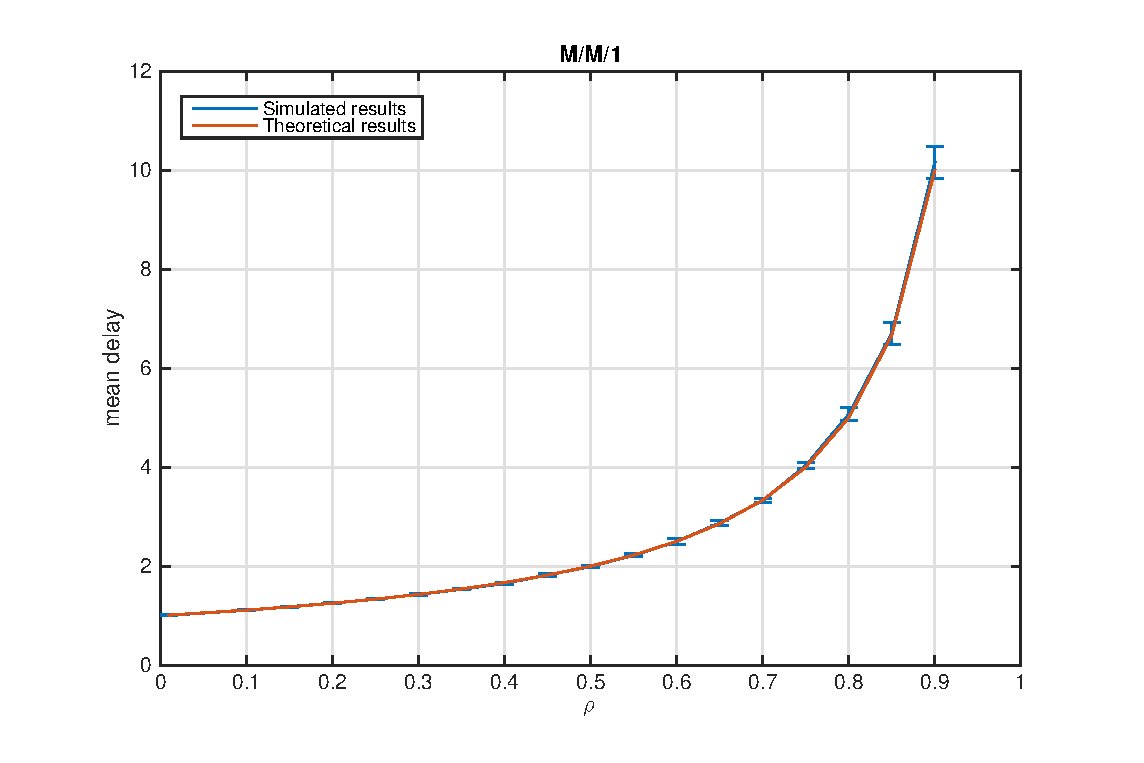
\includegraphics[width = 0.7\textwidth]{mm1_dl}
	\caption{Delay vs. $\rho$ for an M/M/1 queue, simulated and theoretical results by assuming $\mu = 1$}
	\label{fig:mm1_dl}
\end{figure}

\begin{figure}[h!]
	\centering
	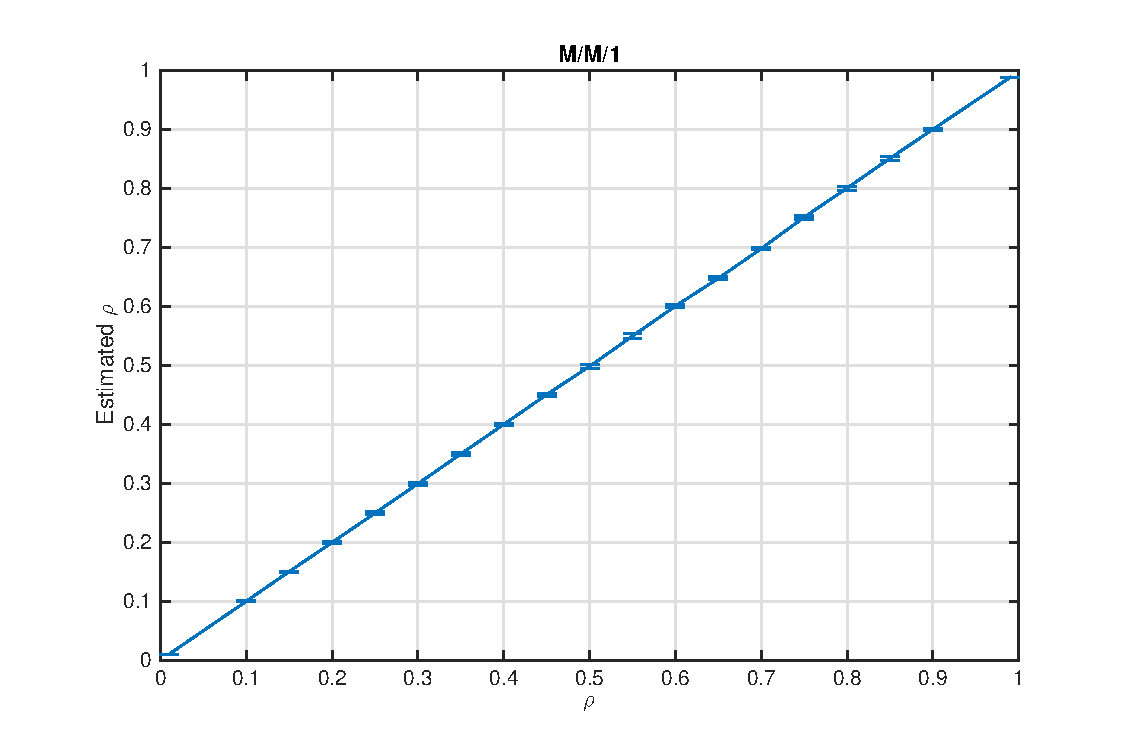
\includegraphics[width = 0.7\textwidth]{mm1_rho}
	\caption{$\hat{\rho}$ vs. $\rho$ for an M/M/1 queue}
	\label{fig:mm1_rho}
\end{figure}

The M/G/1 queue under analysis has Poisson arrivals and service time in 1 or 2 slots with the same probability. Given the duration $l_{slot}$ of a slot the mean length of a service time is then $m_y = 1.5 l_{slot}$, while the variance is $\sigma_y^2 = 0.25 l_{slot}^2$. Then the rate of arrivals is $\lambda = \rho/m_y$. The theoretical average delay in slots from~\cite{bz} is
\begin{equation}
	m_d = \frac{m_y}{2} + \frac{m_y + \lambda \sigma_y^2}{2(1- \lambda m_y)}
\end{equation}

The results of the simulation and comparison with the theoretical curve is in Figure~\ref{fig:mg1_dl}. The slot length is normalized to 1, therefore $l_{slot} = 1$. Figure~\ref{fig:mg1_rho} shows the estimated utilization factor against the theoretical one.

\begin{figure}[h!]
	\centering
	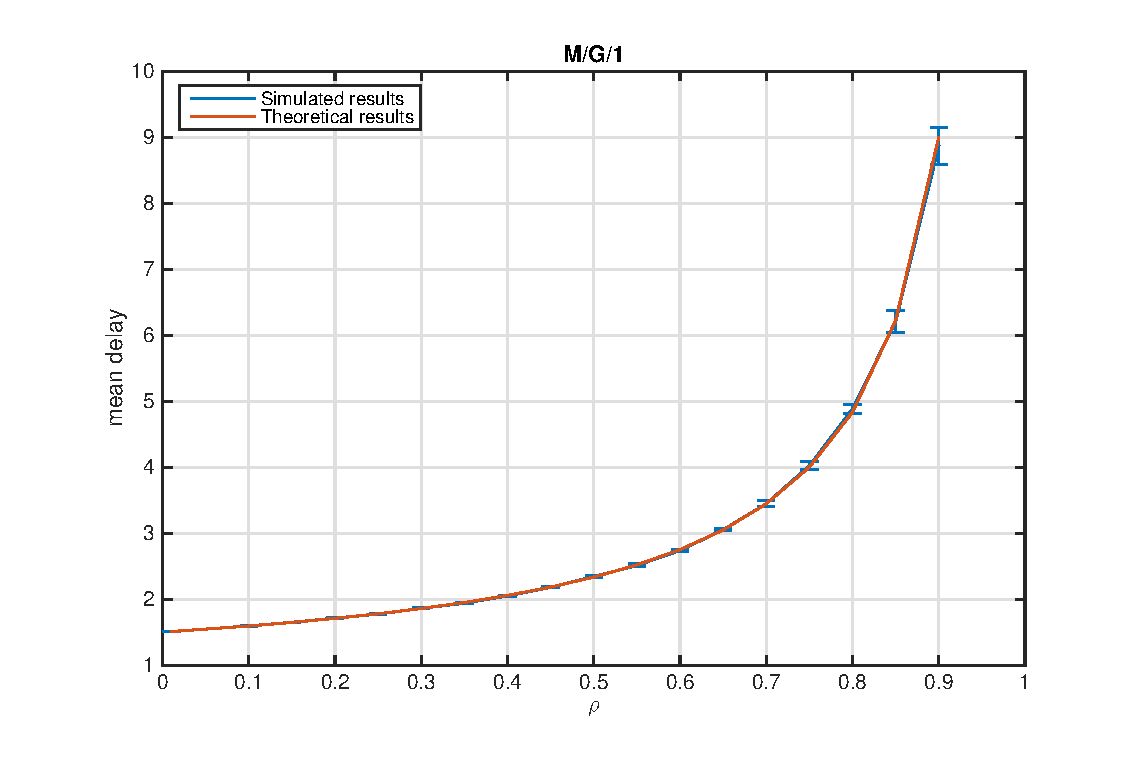
\includegraphics[width = 0.7\textwidth]{mg1_dl}
	\caption{Delay vs. $\rho$ for the described M/G/1 queue given $l_{slot} = 1$}
	\label{fig:mg1_dl}
\end{figure}

\begin{figure}[h!]
	\centering
	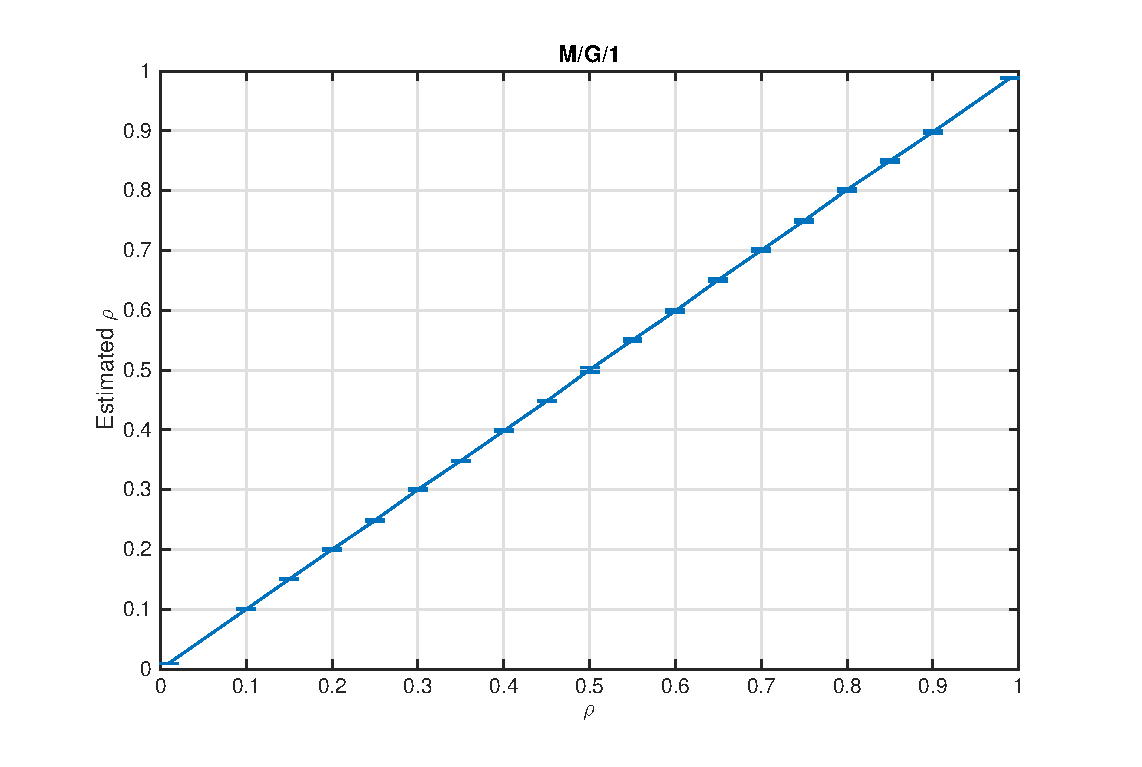
\includegraphics[width = 0.7\textwidth]{mg1_rho}
	\caption{$\hat{\rho}$ vs. $\rho$ for an M/G/1 queue}
	\label{fig:mg1_rho}
\end{figure}

Finally the simulation of the geo/geo/1 queue is compared with simulation of the same queue, in a discrete time fashion, which was part of the previous homework, and with the theoretical analysis that is developed below. In each slot (of length 1) there is an arrival with probability $b_a = 0.5$ and a departure (if the queue is not empty) with probability $b_s \in [0.5, 1]$. Note that for these values of $b_s$ the minimum utilization factor is $\rho = 0.5$. 
From now on, for simplicity, $b_s$ will be $b$.

The theoretical analysis starts from considering the system as a Markov Chain, characterized by the number of users which are in the system at the end of each slot. In particular, by assuming that users cannot be served in the same slot in which they arrive, then for state $X_k > 0$ (i.e. when there is at least one user the system) there can be only three transitions:
\begin{equation}
X_{k+1} = 
\begin{dcases}
	X_k - 1, \quad \mbox{wp } 0.5 b \\
	X_k , \quad \mbox{wp } 0.5 \\
	X_k + 1, \quad \mbox{wp } 0.5(1- b) \\
\end{dcases}
\end{equation}
which correspond to the events
\begin{itemize}
\item no arrivals, one departure
\item no arrivals and no departures OR one arrival and one departure
\item one arrival and no departures
\end{itemize}
Instead for $X_k = 0$ the transitions are
\begin{equation}
X_{k+1} = 
\begin{dcases}
	0, \quad \mbox{wp } 0.5 \\
	1, \quad \mbox{wp } 0.5 \\
\end{dcases}
\end{equation}
Let's now compute the steady state distribution of the states, which will be used to average the number of users in the system. Let $\boldsymbol{\pi}$ be the vector of the steady state probabilities and $\mathbf{P}$ the transition probability matrix as follows
\begin{equation}
\mathbf{P} = 
\begin{pmatrix}
	0.5 	& 0.5 	& 0 		& 0			& 	 		&	& \cdots \\
	0.5b 	& 0.5 	& 0.5(1-b) 	& 0 		& 			&	& \cdots \\
	0 		& 0.5b 	& 0.5 		& 0.5(1-b) 	& 0 		&	& \cdots \\
	0 		& 0 	& 0.5b 		& 0.5 		& 0.5(1-b) 	& 0 & \cdots \\
	\vdots 	& \vdots & 			&  			& 			& 	& \vdots \\
\end{pmatrix}
\end{equation} 
Then the steady state distribution is the solution of
\begin{equation}
	\boldsymbol{\pi} = \boldsymbol{\pi} \mathbf{P}
\end{equation}
which corresponds to the following system
\begin{equation}
\begin{dcases}
	\pi_0 = 0.5 \pi_0 + 0.5b \pi_1	\\
	\pi_1 = 0.5 \pi_0 + 0.5 \pi_1 + 0.5 b \pi_2	\\
	\vdots	\\
	\pi_i = 0.5(1-b) \pi_{i-1} + 0.5 \pi_i + 0.5b\pi_{i+1}, \quad i \ge 2	\\
\end{dcases}
\end{equation}
which yields to
\begin{eqnarray*}
	\pi_1 & = & \frac{\pi_0}{b} \\
	\pi_2 & = & \frac{1-b}{b} \pi_1 \\
	\pi_3 & = & \frac{1-b}{b} \pi_2
\end{eqnarray*}
and so on. This means that
\begin{equation}
	\pi_i = \frac{(1-b)^{i-1}}{b^i} \pi_0, \quad i \ge 1
\end{equation} 
and that $\pi_0$ can be computed in the following way
\begin{gather*}
	\sum_{i = 0}^{\infty} \pi_i = 1 \\
	\pi_0 \left( 1 + \sum_{i = 1}^{\infty} \frac{(1-b)^{i-1}}{b^i} \right) = 1 \\
	\pi_0 \left( 1 + \frac{1}{b}\sum_{i = 1}^{\infty} \left(\frac{1-b}{b}\right)^{i-1} \right) = 1 \\
	\pi_0 \left( 1 + \frac{1}{b} \frac{1}{1-\frac{1-b}{b}} \right) = 1 \\
\end{gather*}
and after some algebraic passages 
\begin{equation}
	\pi_0 = \frac{2b -1}{2b}
\end{equation}
The steady state distribution can be used to compute the mean number of users in the system:
\begin{gather*}
	m_x = \sum_{i = 0}^{\infty} i \pi_i \\
	m_x = \sum_{i = 0}^{\infty} i \frac{(1-b)^{i-1}}{b^i} \pi_0 \\
	m_x = \frac{\pi_0}{b} \sum_{i = 0}^{\infty} i \left( \frac{1-b}{b} \right)^{i-1} \\
	m_x = \frac{\pi_0}{b} \frac{b^2}{(2b -1)^2} \\
	m_x = \frac{2b -1}{2b} \frac{b}{(2b -1)^2} \\
	m_x = \frac{1}{2(2b-1)}
\end{gather*}
Finally, by considering the system arrival rate as $\lambda_a = b_a = 0.5$ and using Little's Law it is possible to compute the mean time in the system spent by each user as
\begin{equation}
	m_d = \frac{m_x}{b_a} = \frac{2}{2(2b-1)} = \frac{1}{2b-1}
\end{equation}


The results of the simulations and the theoretical curve for the delay are in Figure~\ref{fig:gg1_dl}, while the estimated utilization factor is in Figure~\ref{fig:gg1_rho}. In Figure~\ref{fig:gg_real} there are 3 realizations of the g/g/1 queue for different $b_s \in [1/3, 1/2, 2/3]$ and $10^4$ slots.

\begin{figure}[h!]
	\centering
	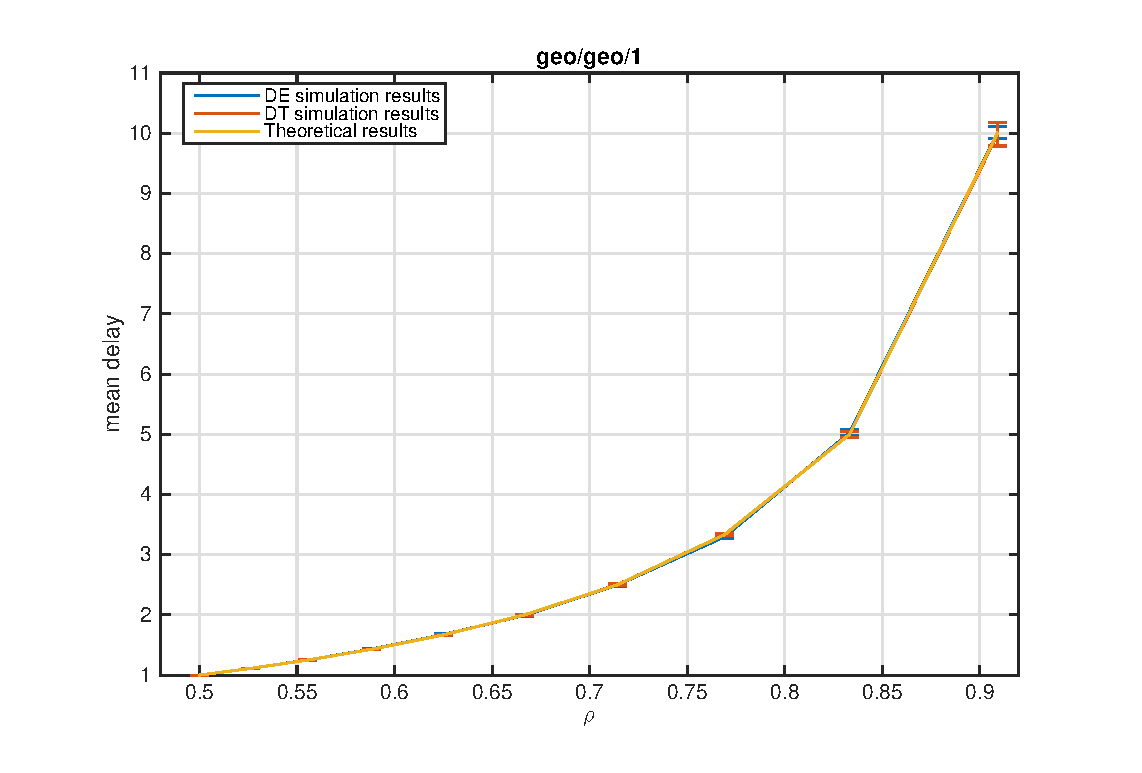
\includegraphics[width = 0.7\textwidth]{gg1_dl}
	\caption{Delay vs. $\rho$ for the described geo/geo/1 queue given $l_{slot} = 1$}
	\label{fig:gg1_dl}
\end{figure}

\begin{figure}[h!]
	\centering
	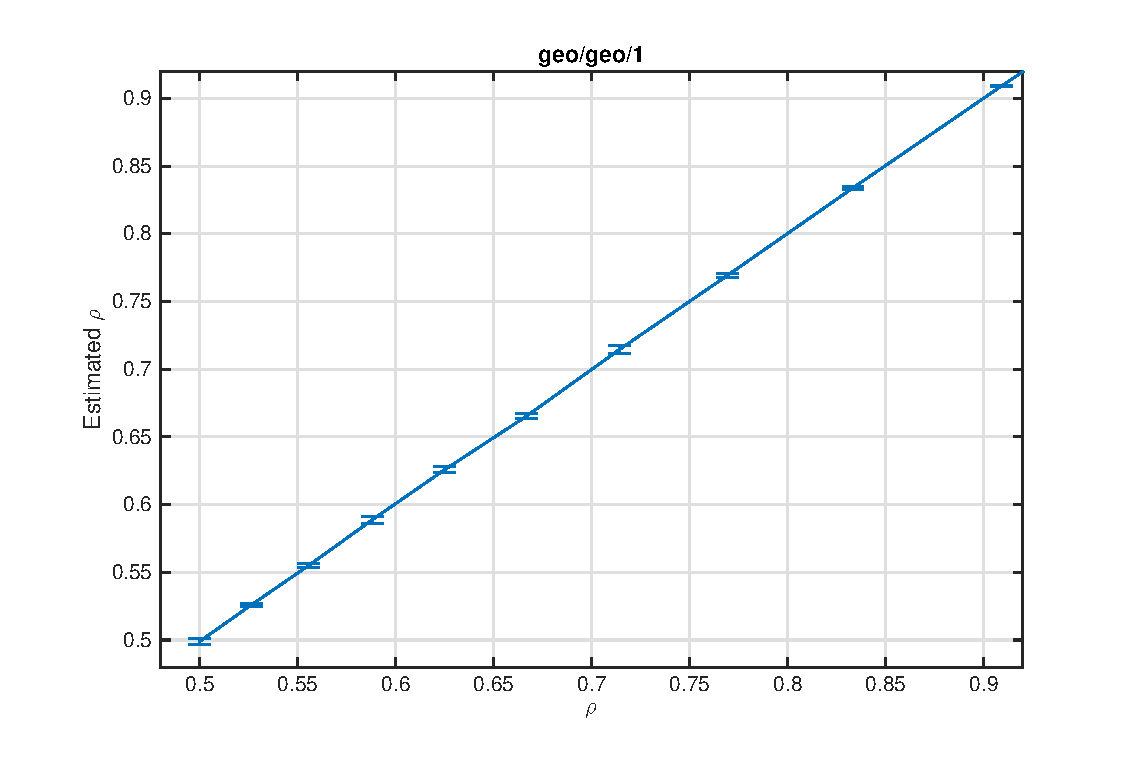
\includegraphics[width = 0.7\textwidth]{gg1_rho}
	\caption{$\hat{\rho}$ vs. $\rho$ for a geo/geo/1 queue}
	\label{fig:gg1_rho}
\end{figure}

\clearpage

\begin{figure}[h!]
	\centering
	\subfigure[$b_s = 2/3$]{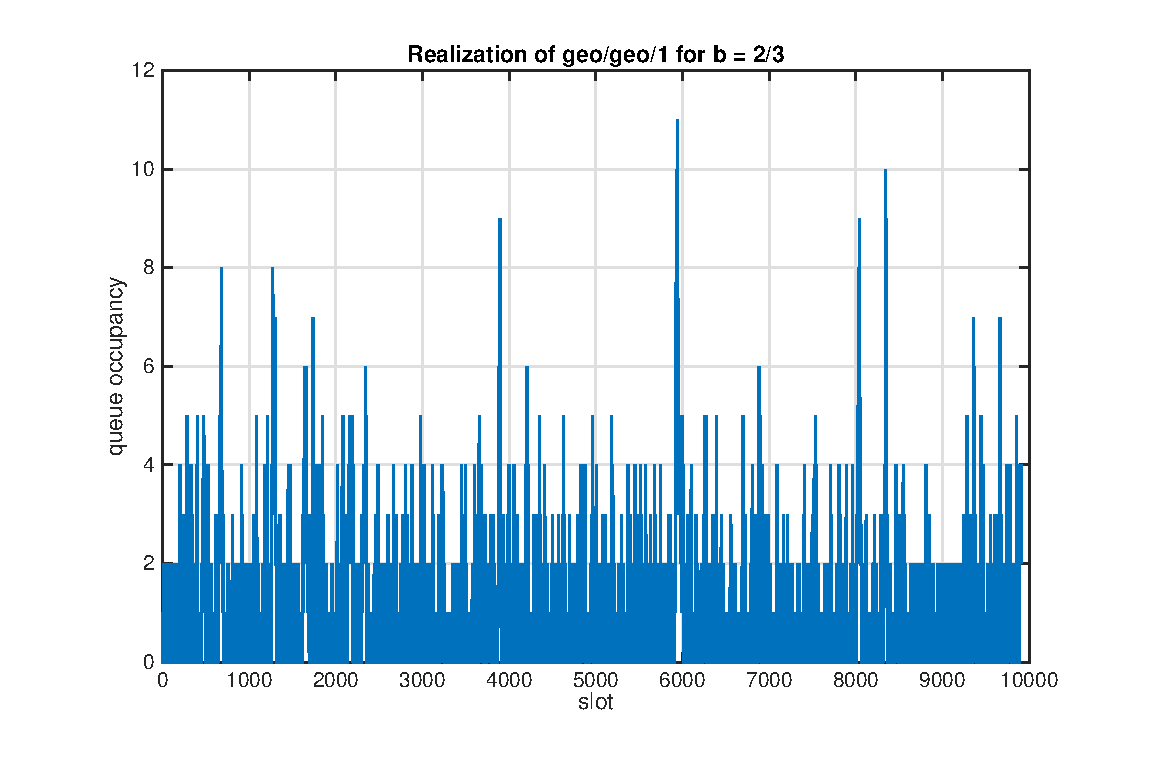
\includegraphics[width=0.45\textwidth]{gg1_066}}
	\subfigure[$b_s = 1/2$]{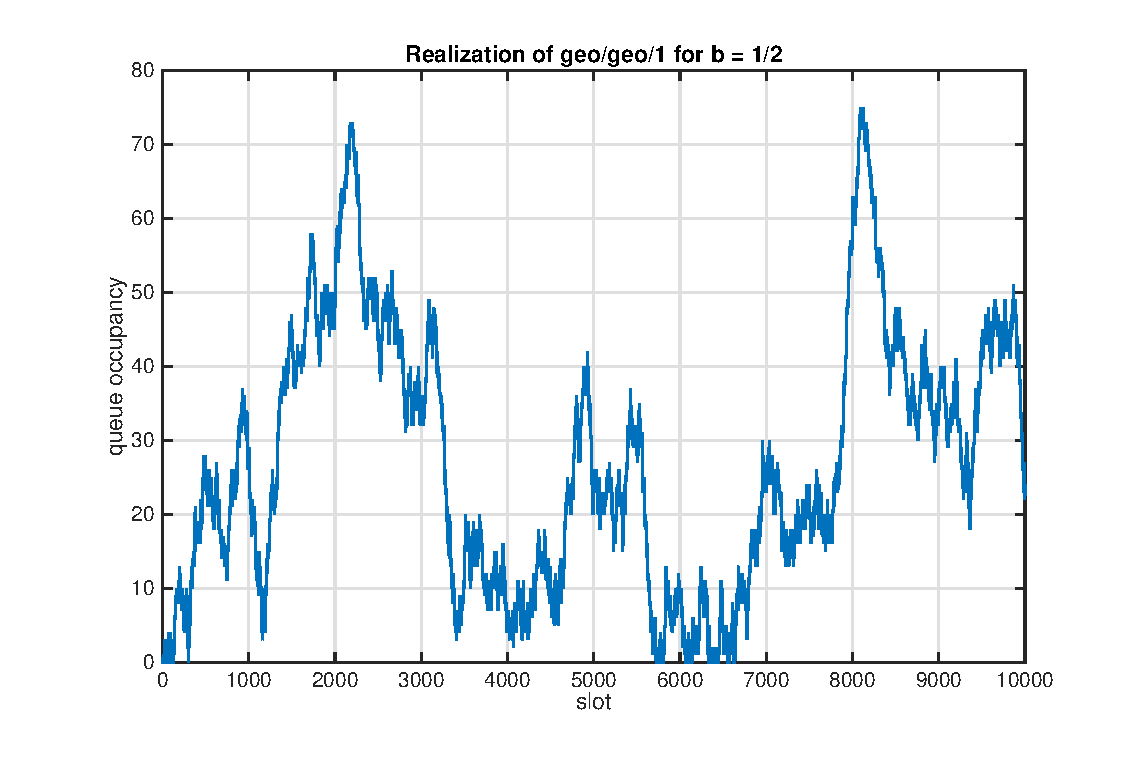
\includegraphics[width=0.45\textwidth]{gg1_05}}
	\subfigure[$b_s = 1/3$]{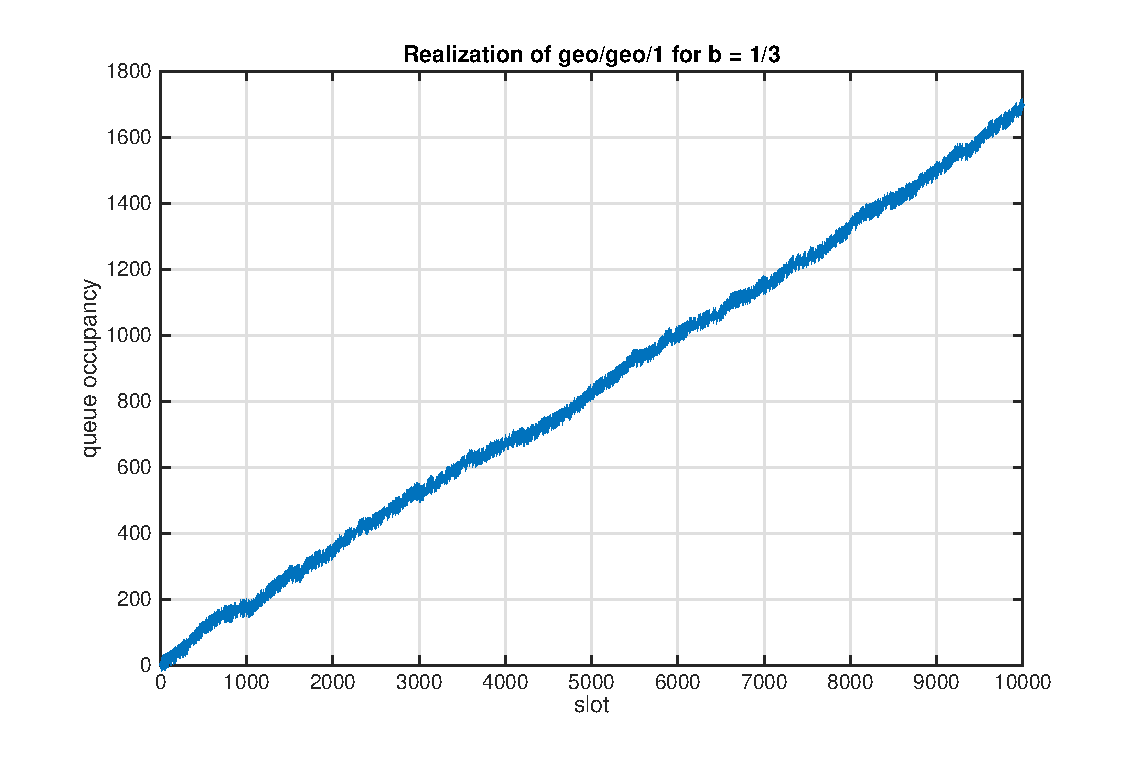
\includegraphics[width=0.45\textwidth]{gg1_033}}
\end{figure}



\section*{Exercise 2 - Read logs and analyze data}
In this second exercise the goal is to extract a look-up table from a log file of a simulator and use it to compute some measurements on useful quantities in underwater optical communications. In particular, the log files are obtained from the simulations of the ambient light irradiance $E_0$ with the simulator HYDROLIGHT. From the 3 different dump files (each for a different value of $c \in [0.15, 0.4, 2.19]$ with $c$ the attenuation coefficient) I recovered the values of $E_0$ and the corresponding depth $z$ in meters using a \texttt{perl} script, which I provide in the attached code. It uses a regular expression to identify the right rows of the log and selects the columns with the desired values with a typical \texttt{perl} construct. In Figure~\ref{fig:e0zm} $E_0$ is plotted as a function of the depth $z$.

\begin{figure}[h!]
	\centering
	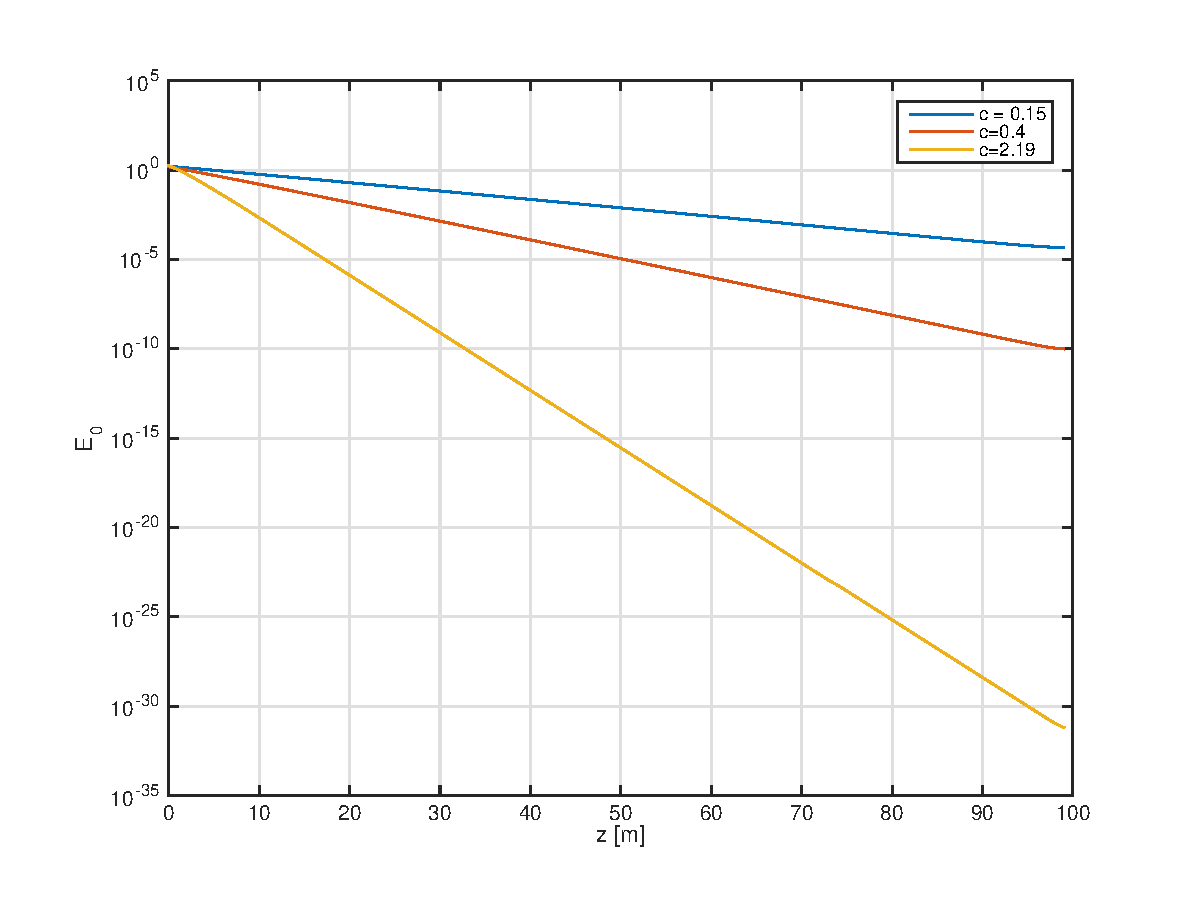
\includegraphics[width = 0.6\textwidth]{e0_z}
	\caption{Irradiance $E_0$ vs. $z$}
	\label{fig:e0zm}
\end{figure}

Some evaluation on the propagation are then carried out with a MATLAB script that uses the provided parameters for receiver and transmitter. The propagation model used is the one proposed in~\cite{optmodel} and assumes that there is a successful transmission if the SNR is over a certain threshold. In particular from the irradiance and the parameters $S$ (sensitivity) and $A_r$ (area of the receiver) of the considered modem it is possible to compute the power of ambient light noise, which is $N_A = (S E_0 A_r)^2$. Let the received power $P$ be
\begin{equation}
	P = \frac{2 P_{tx} A_r \cos(\beta)}{\pi d^2 (1-\cos(\theta)) + 2 A_t}e^{-cd}
	\label{eq:p_opt}
\end{equation}
then the SNR is
\begin{equation}
	\Gamma  = \frac{(SP)^2}{2q(I_D + I_L)BW + \frac{4KTBW}{R} + N_A}
	\label{eq:snr_opt}
\end{equation}
In the following, if the SNR is above the threshold of 20 dB then there is a successful transmission. In particular, by setting the threshold and a distance $d = 10$ m, by inverting~\eqref{eq:snr_opt} in order to get $P$ and~\eqref{eq:p_opt} in order to compute $P_{tx}$ it is possible to know which is the minimum transmission power that can be used to reach a distance $d$. In Figure~\ref{fig:ptx}[a] there is the plot of the minimum $P_{tx}$ against the irradiance $E_0$ for $d = 10$ m, while in Figure~\ref{fig:ptx}[c] the x axis is the depth $z$ considered. Figure~\ref{fig:ptx}[b] shows instead the same as Figure~\ref{fig:ptx}[a] but with a logarithmic x axis, in order to visualize the behavior of the required transmitted power for very low values of $E_0$. It is interesting to note that for $E_0$ below a threshold of about $10^{-4}$ the required power is constant.

\begin{figure}[h!]
	\centering
	\subfigure[$P_{tx}$ to reach $d = 10$ m as a function of $E_0$]{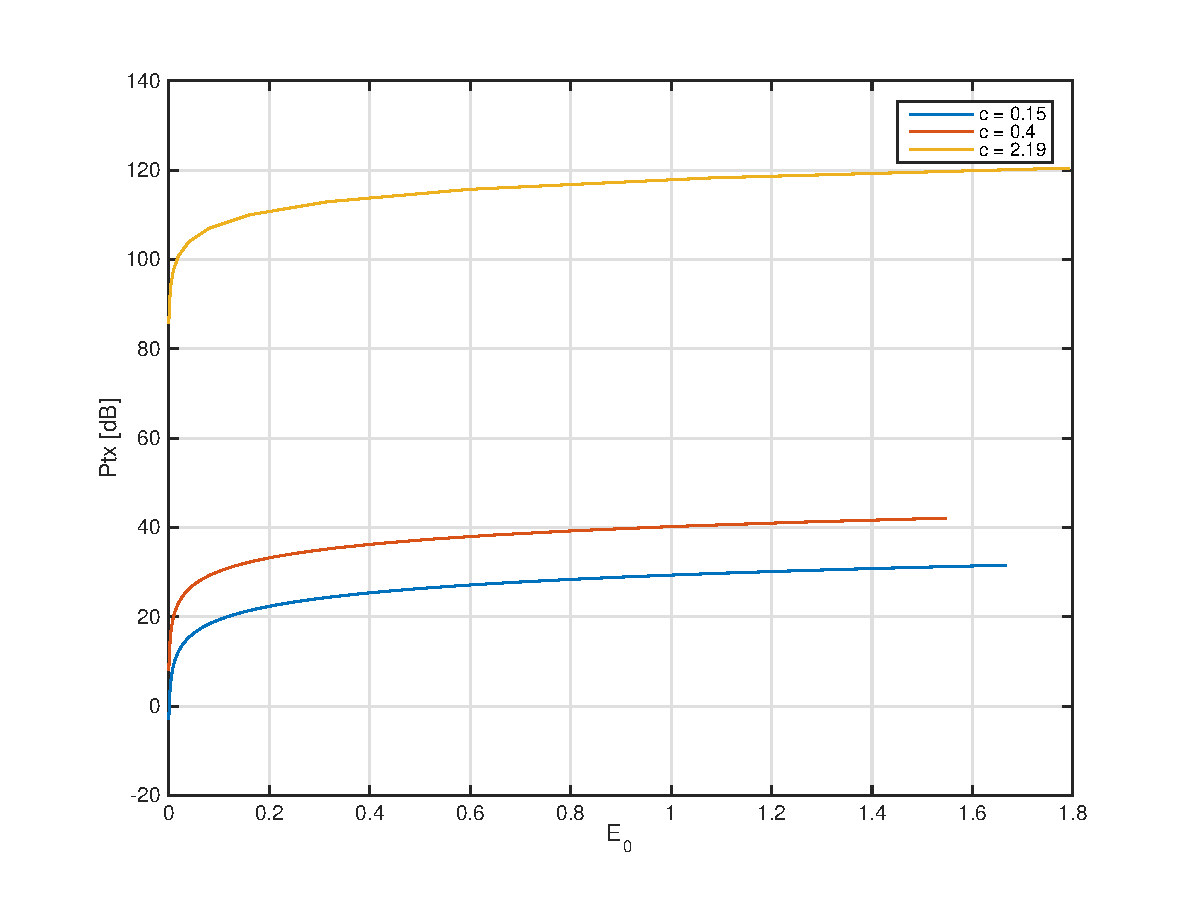
\includegraphics[width = 0.45\textwidth]{ptx_e0}}
	\subfigure[$P_{tx}$ to reach $d = 10$ m as a function of $E_0$, with logarithmic x axis]{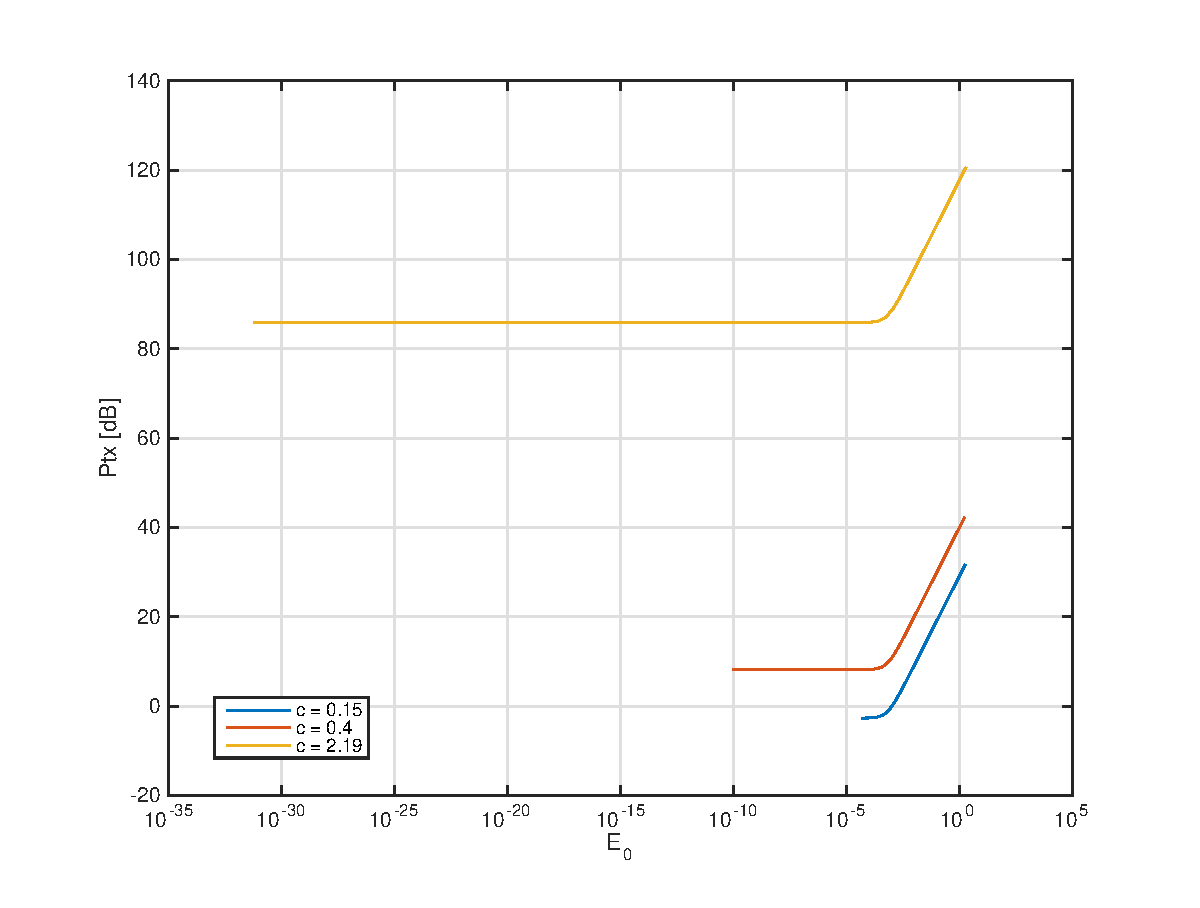
\includegraphics[width = 0.45\textwidth]{ptx_e0_log}}
	\subfigure[$P_{tx}$ to reach $d = 10$ m as a function of $z$]{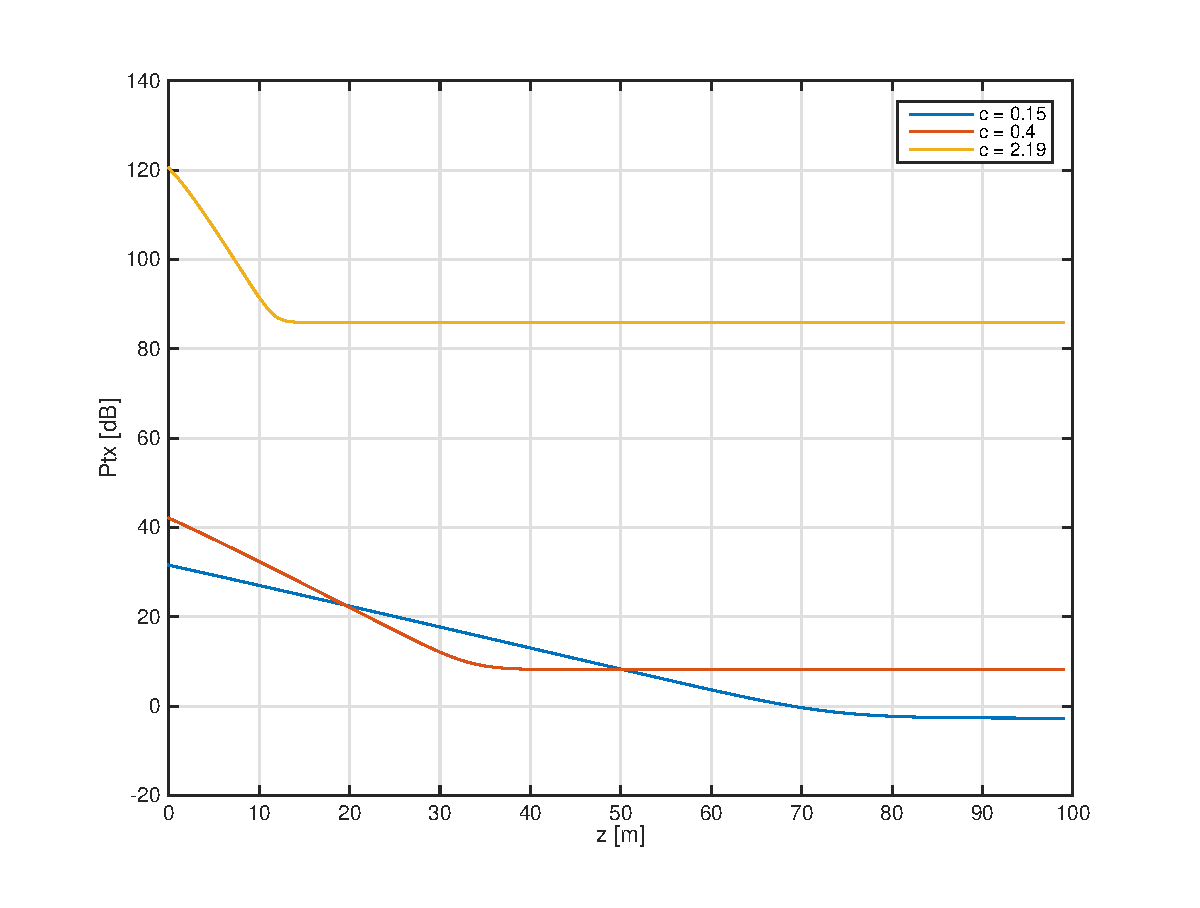
\includegraphics[width = 0.45\textwidth]{ptx_z}}
	\caption{Transmitted power $P_{tx}$ required to transmit at a distance of $d = 10$ meters}
	\label{fig:ptx}
\end{figure}

\clearpage

Finally, the transmit power is set to $P_{tx, max} = 100$ W and the maximum distance at which is possible to transmit is evaluated. Note that~\eqref{eq:p_opt} is not invertible with respect to the distance $d$, therefore the received power $P$ given by~\eqref{eq:p_opt} is precomputed for $d \in [0, 50]$ m and stored in a vector \texttt{P\_d}. Then, given a certain $E_0$, from~\eqref{eq:snr_opt} the minimum received power to guarantee an SNR of 20 dB is computed and the closest $P$ in \texttt{P\_d} is found. The corresponding value of $d$ is chosen as the maximum distance $d_{max}$ at which it is possible to transmit with $P_{tx, max} = 100$ W and that $E_0$ - or the corresponding $z$.

The results are in Figure~\ref{fig:dmax}. Figure~\ref{fig:dmax}[b] is the same as Figure~\ref{fig:dmax}[a] but with a logarithmic x axis, and it shows a behavior which is consistent with Figure~\ref{fig:ptx}[b].

\begin{figure}[h!]
	\centering
	\subfigure[$d_{max}$ as a function of $E_0$, for $P_{tx, max} = 100$]{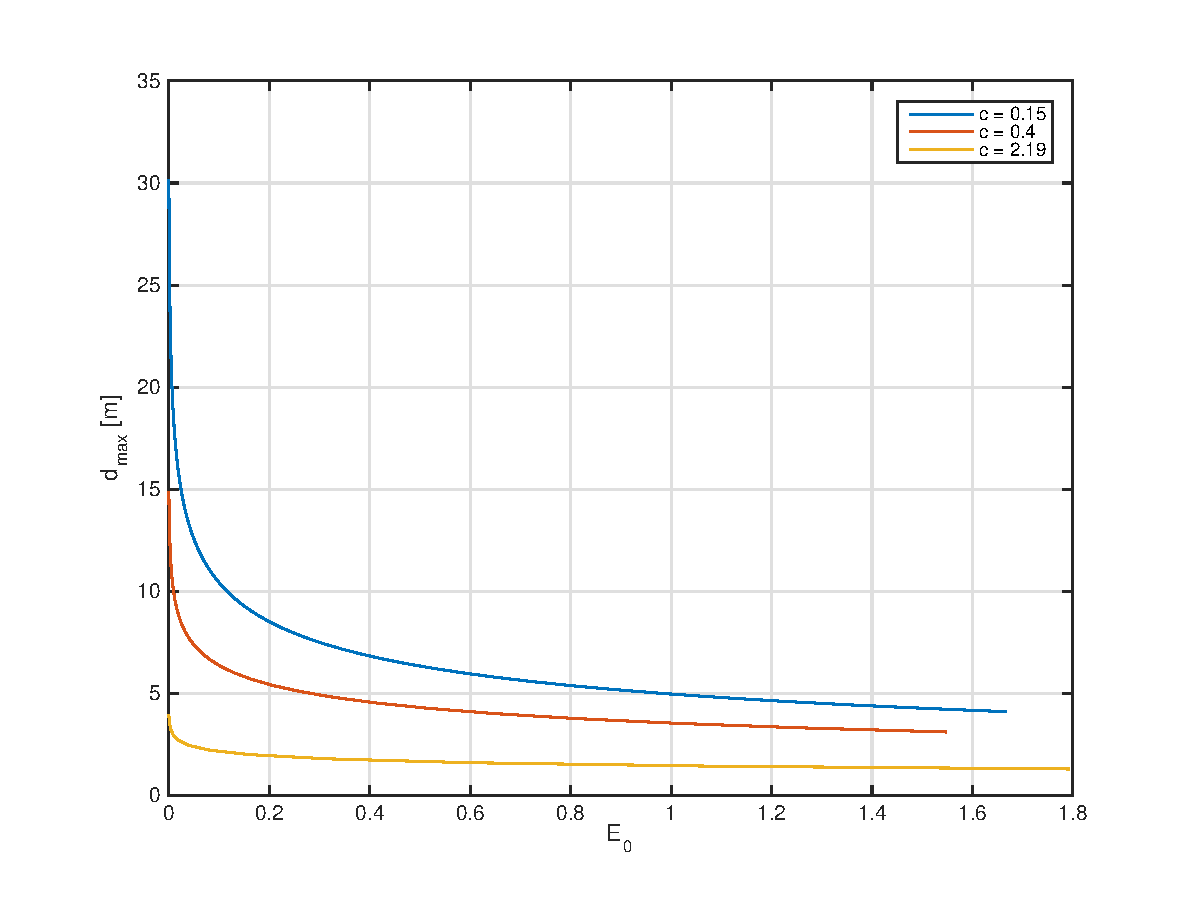
\includegraphics[width= 0.45\textwidth]{dmax_e0}}
	\subfigure[$d_{max}$ as a function of $E_0$ with a logarithmic x axis, for $P_{tx, max} = 100$]{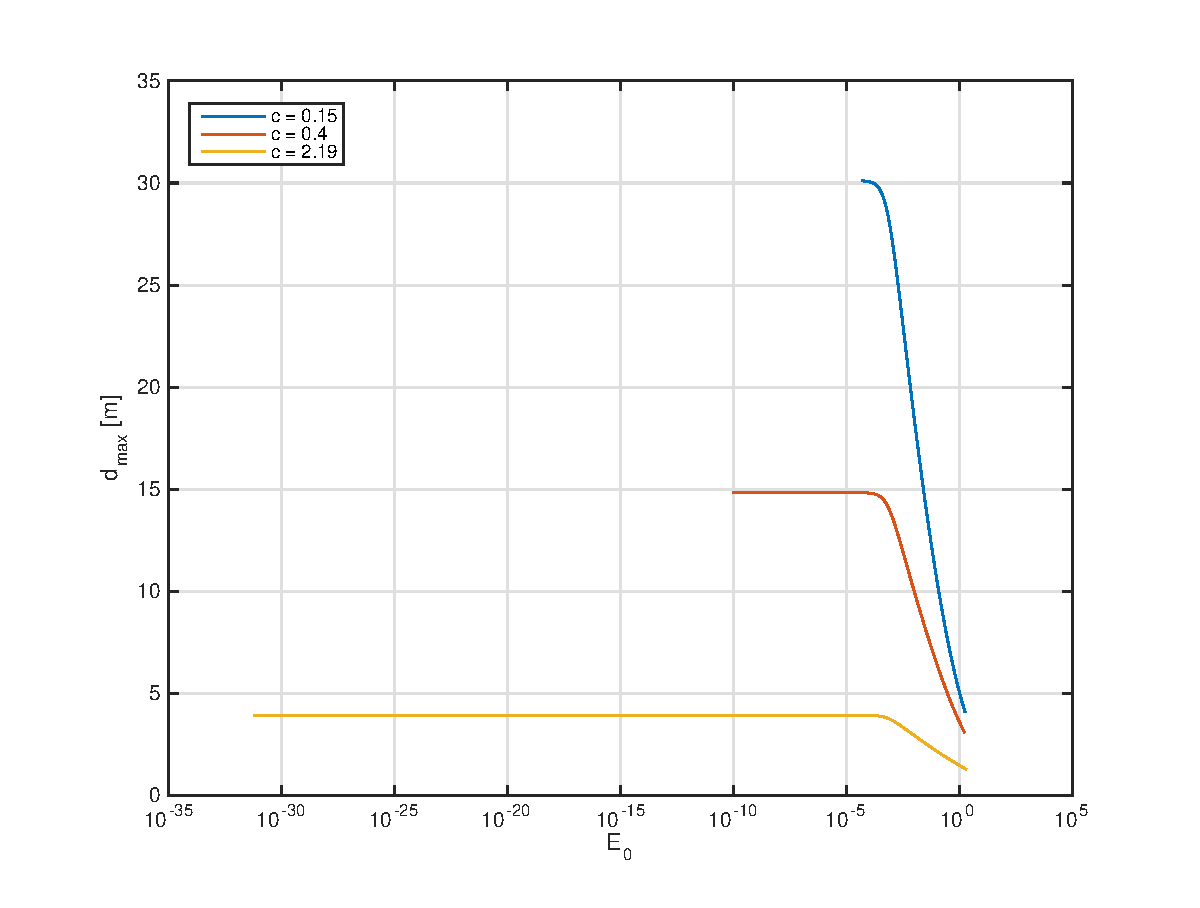
\includegraphics[width= 0.45\textwidth]{dmax_e0_log}}
	\subfigure[$d_{max}$ as a function of $z$, for $P_{tx, max} = 100$]{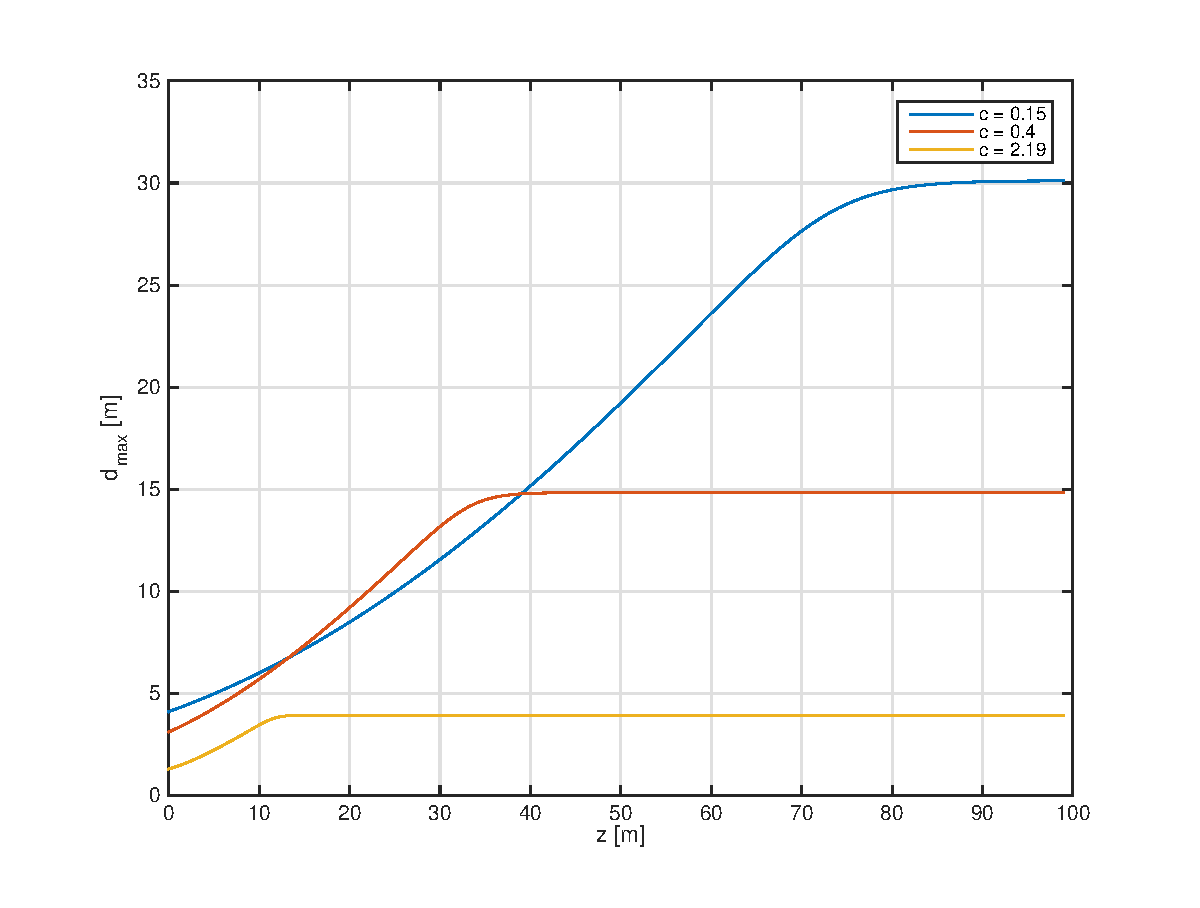
\includegraphics[width= 0.45\textwidth]{dmax_z}}
	\caption{Maximum distance $d_{max}$ with a transmit power of $P_{tx, max} = 100$}
	\label{fig:dmax}
\end{figure}


\begin{thebibliography}{10}

\bibitem{law}
A.M. Law, Simulation Modeling and Analysis, 4th ed., McGraw Hill, 2006

\bibitem{bz}
N. Benvenuto, M. Zorzi, Principles of communications networks and systems, Wiley, 2011

\bibitem{leb}
Y. Le Boudec, Performance Evaluation of Computer and Communications Systems, EPFL, 2015

\bibitem{optmodel}
D. Anguita et al., Optical wireless underwater communication for AUV: Preliminary simulation and experimental results, in Proc. IEEE/OES Oceans, Santander, Spain, Jun. 2011

\end{thebibliography}

\end{document}
